\documentclass[../../00_Main/Main.tex]{subfiles}
\begin{document}

This section describes all the components, the architectures, particular set of parameters and so on, all the stuff that is used to perform the experiments or to detail all that was produced for this work.

\subsection{Phantom-Head Modeling}
%-----------------------------------------------------------
% Phantom-Head Modeling
%-----------------------------------------------------------
\begin{figure}[h]
    \centering
    \begin{subfigure}[b]{0.4\textwidth}
        \centering
        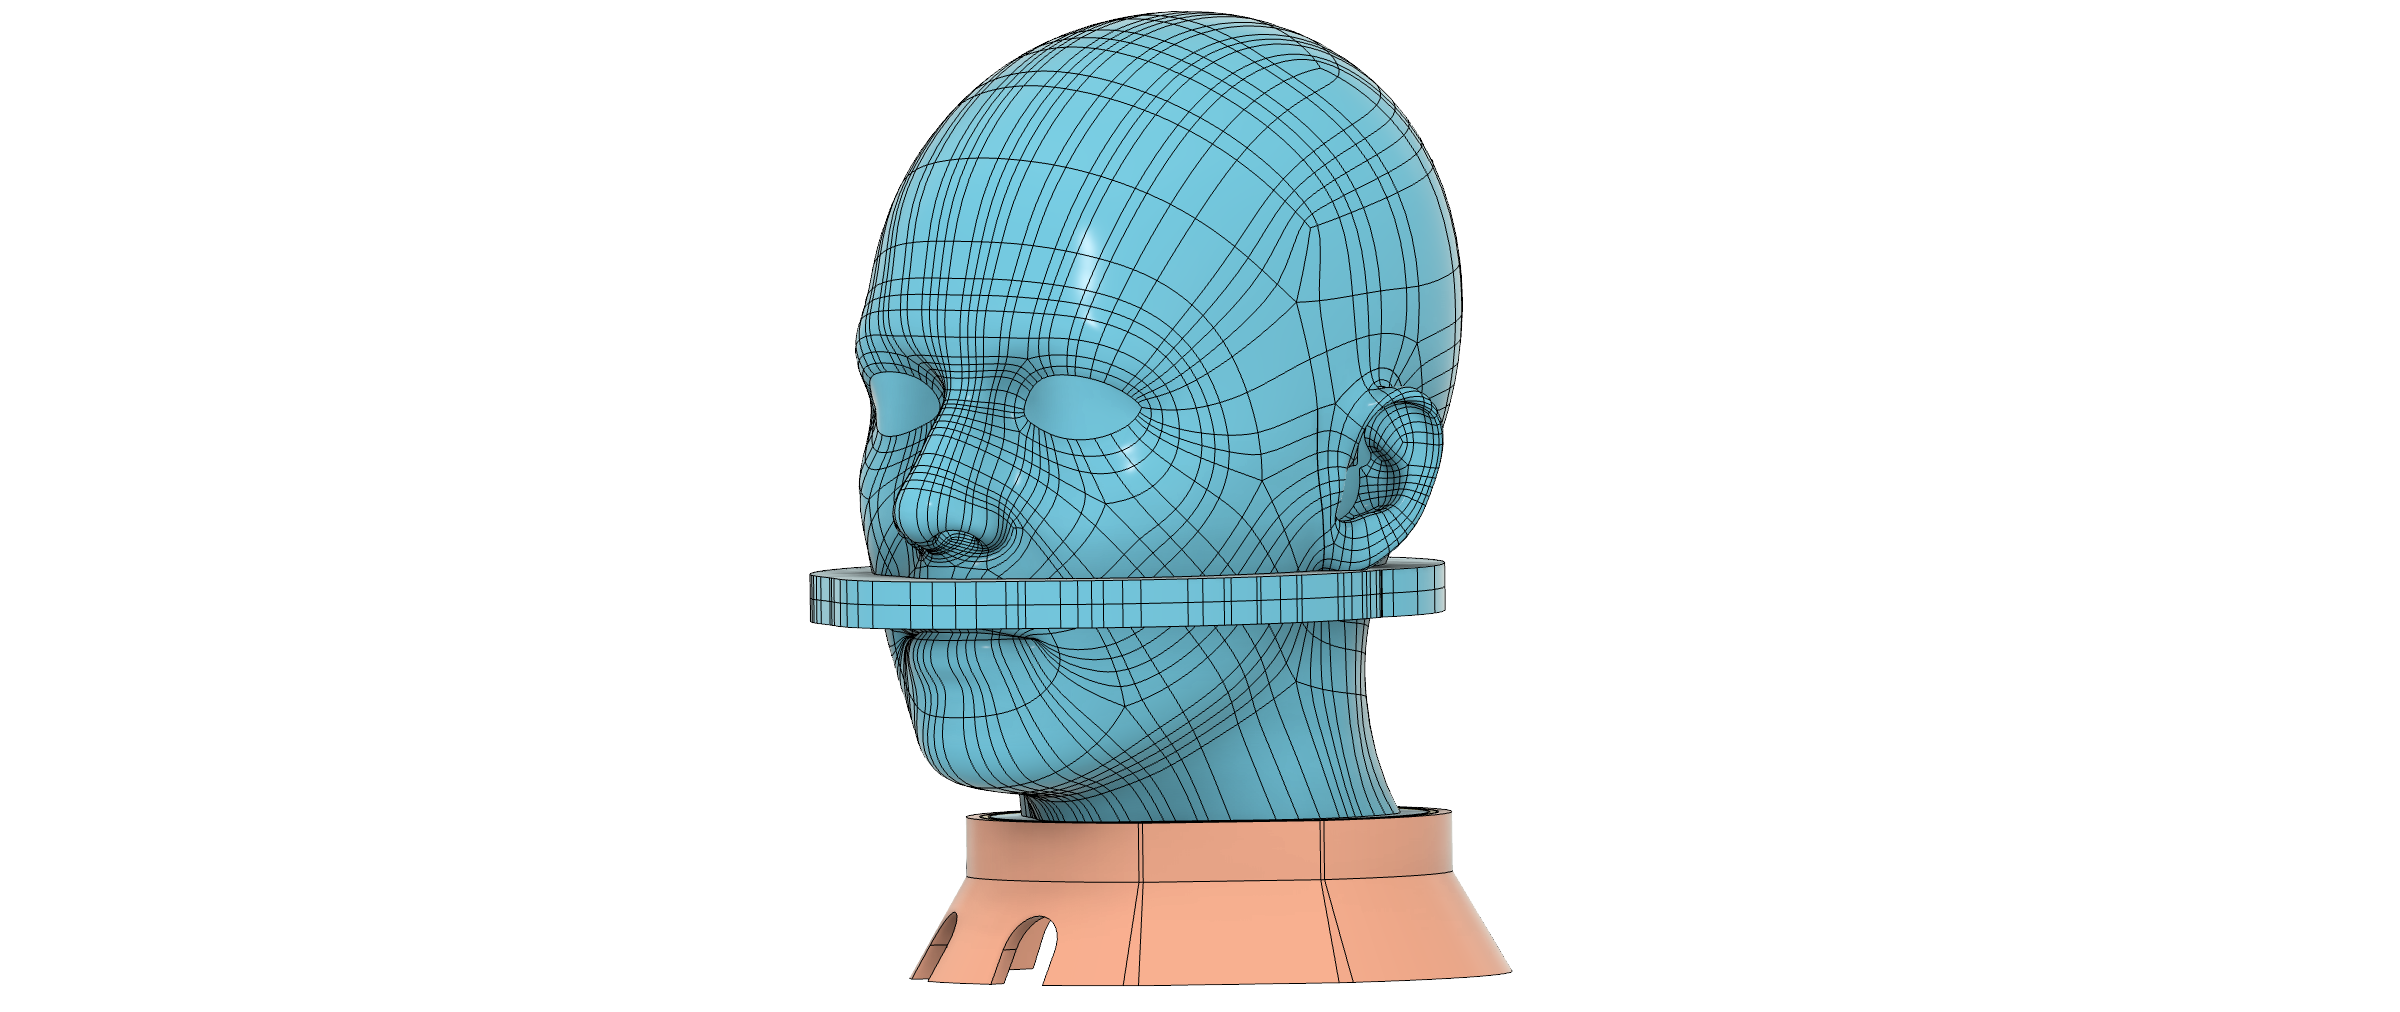
\includegraphics[width=\textwidth]{../../02_Images/3dmodel_overview.png}
        \caption[Phantom assembly exterior]{External overview of the phantom head assembly.}
        \label{fig:head_overview_complete}
    \end{subfigure}
    \hfill
    \begin{subfigure}[b]{0.4\textwidth}
        \centering
        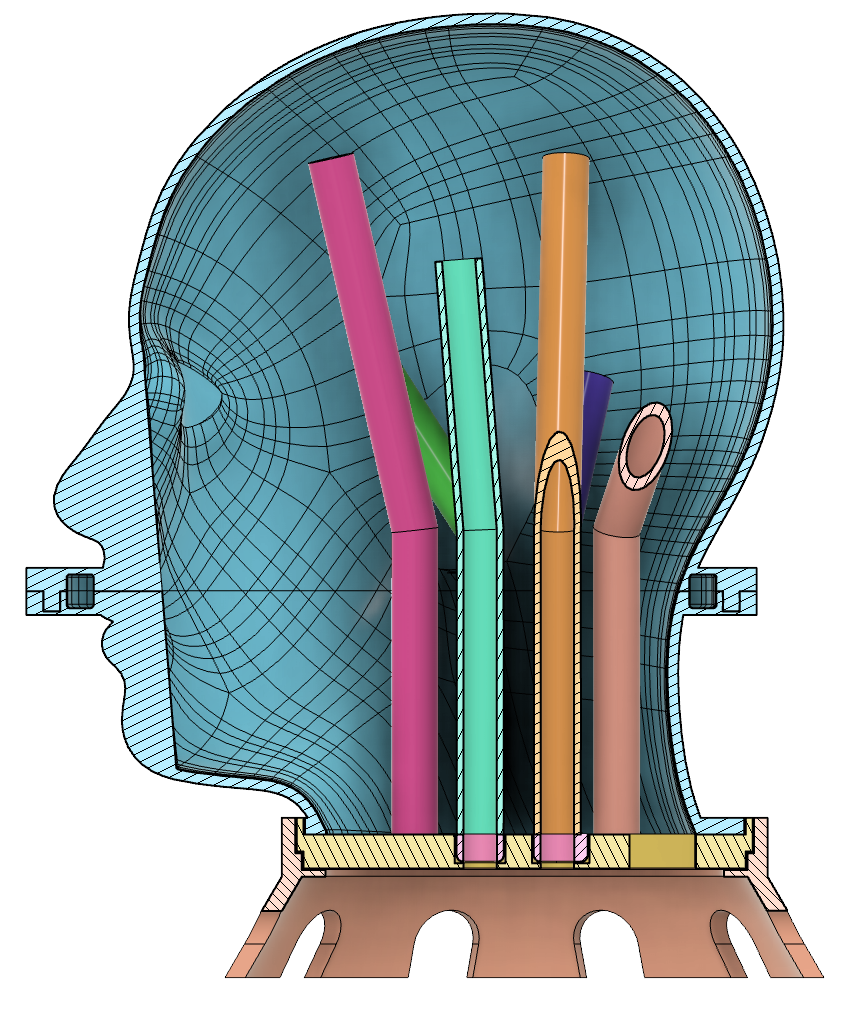
\includegraphics[width=\textwidth]{../../02_Images/3dmodel_section.png}
        \caption[Phantom assembly section]{Section analysis showing internal component disposition.}
        \label{fig:head_overview_section}
    \end{subfigure}
    \caption[Phantom head 3D model]{3D model of the phantom head, highlighting major components and internal structure.}
    \label{fig:head_overview}
\end{figure}

The phantom head model was developed to provide a realistic and modular platform 
for simulating electrical propagation through cranial tissues. 

A realistic mannequin head and torso geometry was sourced from the GrabCAD 
Community Library~\cite{grabcad}. The specific CAD model~\cite{mannequin-model} 
was then imported into \textit{Autodesk Fusion~360} for geometric processing and adaptation.

The phantom assembly was conceived as a modular system. The main components are:

\begin{itemize}
    \item a two-part outer \textbf{head shell} representing the skull boundary and defining the internal cavity to be filled with conductive material,
    \item a set of nine internal \textbf{wire guides} routed toward predefined internal coordinates,
    \item a \textbf{lid} featuring keyed openings for the placement and alignment of the wire guides, and
    \item a \textbf{support base} that seats the lid, provides mechanical stability for the assembly, and includes pass-through openings for routing external cables or connections beneath the phantom.
\end{itemize}


A central principle in the phantom’s design is modularity — the capacity to replace, extend, or reconfigure individual components without rebuilding the entire system. This flexibility is essential for experimental workflows, where electrode layouts, internal coordinates, or stimulation approaches may change between studies. The phantom therefore supports a wide range of experimental configurations and can be easily adapted by other researchers who wish to explore alternative wire-guide layouts, modify the number of guides, or introduce custom access features.

Two aspects of the physical design enable this modularity:

\begin{itemize}
    \item \textbf{Connector base geometry:}  
    The raw parametric model of the connector base for wire guides is provided as a standalone component. New wire guides can be generated by extending this base with a custom tube geometry leading to any desired internal coordinate. This makes it possible to produce alternative guide networks without altering the head shell or the remaining assembly.

    \item \textbf{Interchangeable lid:}  
    An empty version of the inferior lid is included, containing only the mating interface with the shell. Researchers may modify this lid to implement arbitrary numbers of openings or layouts while preserving compatibility with the rest of the phantom.
\end{itemize}


\subsection{Model Overview}
%-----------------------------------------------------------
% Model Overview
%-----------------------------------------------------------

The mannequin geometry was processed to create a shell with a uniform wall thickness of 3.2 mm in the area encompassing the 21 probes according to the the ten-twenty electrode system of the International Federation~\cite{klem-1999}. 
This shell was divided into two interlocking halves (superior and inferior) to simplify printing, 
assembly, and internal inspection.

The internal cavity was designed to be filled with a gelatine-salt-water solution. This space establishes the physical domain where the internal antennas and wire guides are embedded, allowing the propagation of electrical fields to be studied under controlled conditions (see Section~\ref{sec:gelatine-props}). \nota{la seccion ref aca deberia ser una seccion sobre la gelatina, sus propiedades, composicion, etc pero todavia no existe, chequear despues}

Dedicated openings were integrated into the lid to facilitate gel pouring and the alignment 
of the internal wire-guides.

\begin{figure}[h]
    \centering
    \includegraphics[width=0.65\textwidth]{figures/head_shell_overview.png}
    \caption{Overall 3D model of the phantom head assembly, highlighting major components.}
    \label{fig:head_shell_overview}
\end{figure}

\nota{INCLUIR IMAGEN DE TODO EL MODELO DESPUES. Tengo que hacerle una base para que no se caiga y tenga lugar abajo de la lid y arriba de la mesa para sacar los cables por adentro.}


\subsection{Head Shell}
\label{subsec:head_shell}
%-----------------------------------------------------------
% Head Shell
% \label{subsec:head_shell}
%-----------------------------------------------------------

The outer shell constitutes the main structural boundary of the phantom. 
It reproduces realistic cranial curvature while maintaining manufacturability for 3D printing. 
A nominal wall thickness of \nota{t = 3.2~mm (to be confirmed)} 
was applied in the \textit{measuring region}, which corresponds to the area encompassing the 
21 electrode positions defined by the international 10–20 EEG system. 
Outside this region, the geometry was locally thickened or simplified as needed to ensure 
mechanical robustness and facilitate assembly. 
Consequently, the shell is not uniformly thick across its surface, but its 
functional behavior within the measuring area remains consistent and well controlled.

The head was divided into two parts along a \textit{superior–inferior} direction, 
resulting in an upper and a lower half rather than a mid-sagittal or planar cut. 
The separation interface was carefully positioned to remain outside the measuring region, 
thereby preventing any discontinuity or mechanical seam from affecting the probe area. 
Its geometry was shaped to ensure proper mating and alignment between both halves, 
while providing sufficient clearance to minimize potential border effects 
and to facilitate assembly and internal access.

\begin{figure}[h]
    \centering
    \includegraphics[width=0.65\textwidth]{figures/head_shell_sections.png}
    \caption{Head shell showing the two-part split and uniform wall thickness.}
    \label{fig:head_shell_sections}
\end{figure}

\nota{IMAGENES DEL CORTE DE LA CABEZA + MATING STRUCTURES PARA EL CERRADO}


\subsection{Wire Guides}
\label{subsec:wire_guides}
%-----------------------------------------------------------
% Wire Guides
% \label{subsec:wire_guides}
%-----------------------------------------------------------

A network of internal wire guides was designed to route and align the antenna conductors within the gel volume. 
Each guide follows a unique, non-overlapping path leading to a carefully selected endpoint inside the cavity. 
The endpoints were positioned to intentionally break possible spatial symmetries in electrical stimulation, 
thereby enabling more representative and diverse field distributions during testing.

All guides maintain a uniform circular cross-section of \nota{DIAMETER HERE} 
to accommodate a range of cable or electrode diameters. 
This geometry also facilitates easy insertion and sealing of the antennas by any preferred method, 
without requiring a predefined connector or cap design. 
The open-ended approach ensures compatibility with various electrode terminals and sealing techniques.

Each guide is uniquely shaped and numbered at its base for unambiguous identification 
during assembly. 
The numbering system allows consistent correspondence with the experimental layout, \nota{have to decide if we put the numbers on the lid, or provide a diagram for this -- but the guides are id-ed}

The overall design of the wire-guide network enables:
\begin{itemize}
    \item straightforward insertion of flexible antenna wires,
    \item precise alignment of electrode tips within the conductive medium,
    \item and reliable mechanical fixation during gel solidification.
\end{itemize}

\begin{figure}[h]
    \centering
    
\includegraphics[width=0.65\textwidth]{figures/wire_guides.png}
    \caption{Wire guides integrated within the head shell, showing unique routing and numbered bases.}
    \label{fig:wire_guides}
\end{figure}

\nota{Agregar fotos del ensemble + cada una + numero + connector maybe}
\nota{Add table listing each wire guide ID, type, and target location.}


\subsection{Modularity and Adaptability}
\label{subsec:modularity}
%-----------------------------------------------------------
% Modularity and Adaptability
% \label{subsec:modularity}
%-----------------------------------------------------------

A central principle in the phantom's design is modularity — the ability to replace, adapt, or extend 
individual components without the need to re-manufacture the entire assembly. 
This approach supports multiple experimental configurations, facilitates rapid prototyping of new geometries, 
and makes the system reusable by other researchers who may wish to test alternative antenna layouts 
or conductive materials.

Examples include:
\begin{itemize}
    \item \textbf{Base connector:} a parametric connector geometry that can be extended or reoriented 
          to reach any desired location within the gel volume. 
          This enables the creation of new antenna types or electrode placements while keeping the rest 
          of the model unchanged.
    \item \textbf{Lid:} located at the lower end of the shell (neck region), it serves as the main interface 
          for filling the internal cavity with the conductive gel and for fixing or routing the antenna connectors. 
          The lid can be reprinted with customized openings to accommodate different experimental setups, 
          while a \textbf{base (uncut) version} is provided as a reusable template for future modifications.
\end{itemize}

This modular structure simplifies experimentation and ensures that both hardware and design files 
can be easily adapted or shared, promoting reproducibility and collaborative development.

\begin{figure}[h]
    \centering
    
\includegraphics[width=0.65\textwidth]{figures/base_connector.png}
    \caption{Parametric base connector model extending towards the internal conductive medium.}
    \label{fig:base_connector}
\end{figure}

\nota{agregar imgs desp.}


\subsection{Phantom-Head Simulation}
%-----------------------------------------------------------
% Phantom-Head Simulation
%-----------------------------------------------------------

% Add simulation details here


\subsection{Phantom-Head Transfer Model \& Column-Selection Plan}
%-----------------------------------------------------------
% Phantom-Head Transfer Model & Column-Selection Plan
%-----------------------------------------------------------

This section defines the math for the phantom-head system, and proposes several column-selection algorithms to reduce the number of usable dipoles \textbf{without} breaking the physical constraints (forbidden triads).  
It is written so that the same base matrices can be kept in the repository ($F$, $B$, optional $W$), and each selection algorithm returns a diagonal \emph{selection/mask} matrix $S$ ($36\times 36$) to turn dipoles on/off.

\bigskip

\subsubsection{Short system description}

We have:

\begin{itemize}
  \item \textbf{9 internal electrodes} (``antennas'') whose voltages can be controlled.
  \item \textbf{36 possible dipoles}: every unordered pair $(e_x, e_y)$ with $1 \le x < y \le 9$.
  \item 21 \textbf{scalp probes} measure potentials.
  \item \textbf{A linear, static model} obtained from simulations: \emph{``if dipole $(e_x, e_y)$ is excited with $+1/-1$ V, what do the 21 probes see?''}
\end{itemize}

Goal: keep \textbf{one} master transfer matrix from dipoles to scalp (the original \texttt{F}), and \textbf{one} master matrix from antennas to dipoles (\texttt{B}), and apply \textbf{selection} via a diagonal matrix $S$ that zeroes out non-selected dipoles.

\bigskip

\subsubsection{Unified system equation}

We will use \textbf{one} equation for \textbf{all} cases:

\[
\boxed{
V_{\text{scalp}}^{(w)} \;=\; W \, F \, S \, B \, V_{\text{antena}}
}
\]

where:

\begin{itemize}
  \item $V_{\text{antena}} \in \mathbb{R}^{9\times 1}$:  
  antenna voltage vector; values that can be set on the 9 internal electrodes. Units: V 
  
  \item $B \in \mathbb{R}^{36\times 9}$:  
  \textbf{antenna $\to$ dipole} difference matrix.  
  Each \textbf{row} corresponds to one dipole $(e_x, e_y)$: it has $+1$ in column $x$, $-1$ in column $y$, and $0$ elsewhere.

  \item $S \in \mathbb{R}^{36\times 36}$:  
  \textbf{selection / mask matrix} (diagonal).
  \begin{itemize}
    \item $S_{jj} = 1$: dipole $j$ is \textbf{enabled}.
    \item $S_{jj} = 0$: dipole $j$ is \textbf{disabled}.
  \end{itemize}
  Each selection algorithm returns such an \texttt{S}.

  \item $F \in \mathbb{R}^{21\times 36}$:  
  \textbf{dipole $\to$ scalp} transfer matrix (this is the one already computed from the 36 unit-dipole simulations).  
  Column $j$ of $F$ is the 21-probe response to dipole $j$ excited with $\pm 1$ V.

  \item $W \in \mathbb{R}^{21\times 21}$:  
  \textbf{probe-weighting} matrix (diagonal).
  \begin{itemize}
    \item $W = I_{21}$ $\to$ unweighted model
    \item $W \neq I_{21}$ $\to$ emphasize/de-emphasize regions (frontal, occipital, etc.)
  \end{itemize}

  \item $V_{\text{scalp}}^{(w)} \in \mathbb{R}^{21\times 1}$:  
  weighted scalp voltages predicted by the model.
\end{itemize}

So, the data flow is:

\begin{enumerate}
  \item \textbf{antennas} $\to$ $B V_{\text{antena}}$ $\to$ \textbf{dipole amplitudes}
  \item dipoles $\to$ $S (B V_{\text{antena}})$ $\to$ \textbf{only allowed/selected dipoles}
  \item selected dipoles $\to$ $F S B V_{\text{antena}}$ $\to$ \textbf{scalp voltages}
  \item scalp voltages $\to$ $W F S B V_{\text{antena}}$ $\to$ \textbf{weighted scalp voltages}
\end{enumerate}

\subsubsection*{Why masking \textbf{B} and not \textbf{F}?}

\begin{itemize}
  \item masking \textbf{B} via $S B$ keeps the original \textbf{F} intact — no duplications;
  \item mathematically:
  \[
  F \, S \, B = F \, (S B)
  \]
  because matrix multiplication is associative;
  \item disabling a dipole means: ``this dipole will \textbf{never} be produced from any antenna voltage'' $\to$ that is naturally a constraint on the \textbf{dipole-generation} side (\texttt{B}), not on the measurement side (\texttt{F});
  \item selection algorithms can therefore \textbf{always} return $S_{alg}$.
\end{itemize}

\bigskip

\subsubsection{Selection algorithms}

All algorithms described below operate on the same base matrices defined previously:
the dipole $\rightarrow$ scalp matrix $F$, the antenna $\rightarrow$ dipole matrix $B$,
and the optional probe weighting matrix $W$.

Each algorithm builds a list of selected dipoles
\(\text{selected} = \{(i,j), (k,l), \dots\}\)
subject to the physical constraint that no forbidden triad
\(\{(i,j), (i,k), (j,k)\}\)
is ever formed.  
The output of each algorithm is a diagonal selection (mask) matrix \(S \in \mathbb{R}^{36\times36}\)
whose diagonal entries are one for selected dipoles and zero otherwise.
The mask \(S\) is applied on the dipole–generation side of the system,
yielding $M = W \cdot F \cdot S \cdot B$ as the effective forward model.

\nota{
For each one, we need a Goal, rationale and procedure
+ any alg specific info
}


\biblio % Needed for referencing to working when compiling individual subfiles - Do not remove
\end{document}